\section{How fast will the complete Raft algorithm elect a leader in
real networks?}
\label{leaderelection:lan}


The previous sections were based on simplified models of how leader
election works in Raft. We wanted to know how fast Raft will be able to
elect a leader in the real world. To find out, this section evaluates
Raft's leader election algorithm using a real-world benchmark in a LAN
environment and a realistic simulator in a slower WAN environment.

\subsubsection{Real-world implementation on a LAN}

\begin{table}
\centering
\begin{tabular}{r l}
code & LogCabin~\cite{logcabin}, written in C++11 \\
OS & x86-64 RHEL6 (Linux 2.6.32) \\
CPU & Xeon X3470 (4 cores, 8 hyperthreads) \\
disk & ext4 file system on Crucial M4 SSDs (1 SSD per server) \\
network & Protocol Buffers~\cite{Varda:2008} over TCP/IP over 1~gigabit Ethernet \\
configuration & in-memory state machine, no log compaction \\
\end{tabular}
\vcaption[experimental setup for benchmark]{
Experimental setup for real-world LAN benchmark.
}
\label{tab:leaderelection:benchmarksetup}
\end{table}

We used LogCabin to measure the performance of Raft's
leader election algorithm on five servers connected by a gigabit Ethernet network.
The experimental setup is summarized in
Table~\ref{tab:leaderelection:benchmarksetup}. The benchmark repeatedly
crashed the leader of a cluster of five servers and timed how long it
took to detect the crash and elect a new leader. The benchmark measured
the time from when the old leader crashed until the other servers
received the new leader's first heartbeat (see
Figure~\ref{fig:leaderelection:nosplit:timeline}). The leader was crashed
randomly within its heartbeat interval, which was half of the
minimum election timeout for all tests. Thus, the smallest possible
downtime was about half of the minimum election timeout.

\begin{figure}
\centering

\begin{subfigure}{\textwidth}
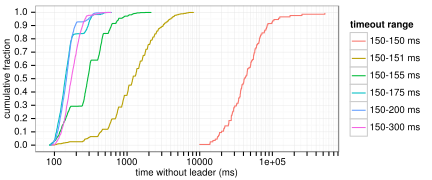
\includegraphics{leaderelection/benchmarks-randomness}
\caption{
Time to elect new leader when varying the range of randomness in
election timeouts.
}
\label{fig:leaderelection:benchmark-randomness}
\end{subfigure}

\vspace{4ex}

\begin{subfigure}{\textwidth}
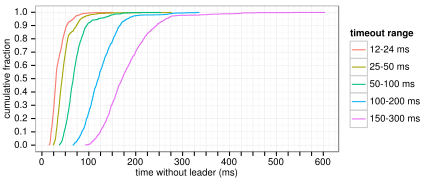
\includegraphics{leaderelection/benchmarks-scale}
\caption{
Time to elect new leader when scaling the minimum election timeout.
}
\label{fig:leaderelection:benchmark-scale}
\end{subfigure}

\vcaption[benchmark results on LAN cluster]{
The graphs show the time to detect and replace a crashed leader in the
real-world LAN benchmark. Each line represents \num{1000}
trials (except for 100 trials for ``\SIrange{150}{150}{\milli\second}'')
and corresponds to a
particular choice of election timeouts; for example,
``\SIrange{150}{155}{\milli\second}''
means that election timeouts were chosen randomly and uniformly between
\SI{150}{\milli\second} and \SI{155}{\milli\second}.
The steps that appear on the graphs show when split votes occur (the
cluster must wait for another election timeout before a leader can be
elected).
The measurements were taken on a cluster of five servers with a
broadcast time (network round trip plus disk write) of roughly
\SI{15}{\milli\second}.
Results for a cluster of nine servers are similar.
}
\label{fig:leaderelection:benchmark}
\end{figure}

The benchmark tried to generate a worst-case scenario for leader
election. First, it synchronized the old leader's heartbeat RPCs before
causing the old leader to exit; this made the follower's election timers
start at approximately the same time, leading to many split votes if the
timeout values were not sufficiently randomized. Second, the servers in
each trial had different log lengths, so two of the four servers were not
eligible to become leader (however, Section~\ref{leaderelection:logsdiff}
will show that this has only a minor effect on election times).

Figure~\ref{fig:leaderelection:benchmark-randomness} shows that elections
complete in under one second when the timeout range is sufficiently
broad. A small amount of randomization in the election timeout is enough
to avoid split votes in elections. In the absence of randomness, leader
election consistently took longer than \SI{10}{seconds} due to many split
votes. Adding just \SI{5}{\milli\second} of randomness helps
significantly, resulting in
a median downtime of \SI{287}{\milli\second}.
Using more randomness improves worst-case
behavior: with a \SI{50}{\milli\second} random range, the worst-case
completion time
(over \num{1000} trials) was \SI{513}{\milli\second}.

Figure~\ref{fig:leaderelection:benchmark-scale} shows that downtime can
be reduced by reducing the election timeout.
With an election timeout of
\SIrange{12}{24}{\milli\second}, it takes only
\SI{35}{\milli\second} on average to elect a leader
(the longest trial took \SI{152}{\milli\second}).
However, lowering the timeouts beyond this point violates Raft's timing
requirement: leaders have difficulty broadcasting heartbeats before
other servers start new elections. This can cause unnecessary leader
changes and lower overall system availability.
We recommend using a conservative election timeout such as
\SIrange{150}{300}{\milli\second};
such timeouts are unlikely to cause unnecessary leader changes, result
in a low rate of split votes, and will still provide good availability.

\subsubsection{Simulated WAN network}

We developed a simulator called AvailSim~\cite{availsim} to
explore a wider range of leader election scenarios. Unlike the
fixed network in our real-world test cluster, AvailSim allows the
latency of the simulated network to be configured arbitrarily.
(We used AvailSim to interactively explore a wide space of leader
election scenarios and algorithms, but this chapter only includes a few
relevant results.)

AvailSim is a close approximation to a complete Raft system, but its
election time results differ from real elections in two ways:
%
\begin{enumerate}
%
\item Each server in AvailSim begins with a fresh election timer. In
practice, the leader will crash at some random point in time between
heartbeats. The election times produced by AvailSim are thus an average
of half a heartbeat interval too large.
%
\item AvailSim does not add any time for processing messages or writing
to disk (these are infinitely fast in the simulator). CPU time should be
short relative to network latency, and disks need not play a significant
role in leader election anyhow (see
Section~\ref{leaderelection:split:total}).
%
\end{enumerate}

\begin{figure}[p]
\centering
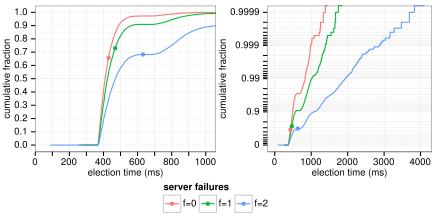
\includegraphics{leaderelection/multi-submission-failures}
\vspace{-4ex}
\vcaption[election performance on a simulated WAN cluster]{
Election performance as calculated by AvailSim for a WAN (one-way
network latency of 
\SIrange{30}{40}{\milli\second}). The figure shows a cluster of
five servers with zero, one, and two servers having failed.
\\
The left graph plots the CDFs of election times. The right graph plots
the same curves on a reverse-logarithmic $y$ axis to magnify
detail on the tail of the distribution. Each CDF summarizes \num{10000}
simulated elections. The point on each curve marks the average election
time.
}
\label{fig:leaderelection:simulation:dist:submission-failures}
\end{figure}

\begin{figure}[p]
\centering
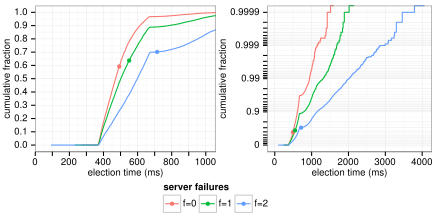
\includegraphics{leaderelection/multi-submission-failures-logsdiff}
\vspace{-4ex}
\vcaption[election performance with differing logs]{
Election performance as calculated by AvailSim when each server has a
different log (using the same WAN configuration as
Figure~\ref{fig:leaderelection:simulation:dist:submission-failures}).
Performance is similar to
Figure~\ref{fig:leaderelection:simulation:dist:submission-failures}, where
the servers' logs are all the same.
}
\label{fig:leaderelection:simulation:dist:submission-failures-logsdiff}
\end{figure}

We used AvailSim to approximate a WAN spanning the continental US. Each
message was assigned a latency chosen randomly from the uniform range of
\SIrange{30}{40}{\milli\second}, and the servers' election timeout range was set
accordingly to \SIrange{300}{600}{\milli\second} (about 10--20 times the
one-way network latency).

Figure~\ref{fig:leaderelection:simulation:dist:submission-failures} shows
how quickly a five-server cluster elects a leader in this WAN
environment. When only one of the five servers has failed, the average
election completes within about
\SI{475}{\milli\second}, and 99.9\% of
elections complete within
\SI{1.5}{\second}. Even when two of the five servers
have failed, the average election takes about
\SI{650}{\milli\second} (about 20
times the one-way network latency), and 99.9\%
of elections complete in
\SI{3}{\second}. We believe these election times are more than adequate for
most WAN deployments.
